\section{Cracking Pattern}
% TODO: GIANNINI(2012) P14-15 (Nothing Much)


\section{Compressive Strength}

\subsection{ASR}


% ALKAN HAFCI(2013) P25 Chapter 3 (Pretty Good!)

In first test study, T. Ahmed et al. used Thames Valley sand (in Mix A), fused silica (in Mix B) and slowly reactive aggregate (in Mix C) to investigate the effect of ASR expansion on compressive strength of concrete. The specimens, 100x100x100 mm in size [BSEN 1290-3, 2000] were cast and cured with respect to BS 1881 Part 122 [BS, 1881]. After casting and moulding, the cube specimens were cured for 28 days in water at 20 0C and then the temperature was increased to 38 0C to accelerate alkali-silica reaction. In this temperature, the specimens were stored at water tank until 12 months passed [Ahmed et al., 2003].After 28-days curing at 20 0C and storage at 38 0C for 12 months, the expansion ratios and compressive strength are given in Table \ref{}.

% TODO: Remake table

\begin{figure}
  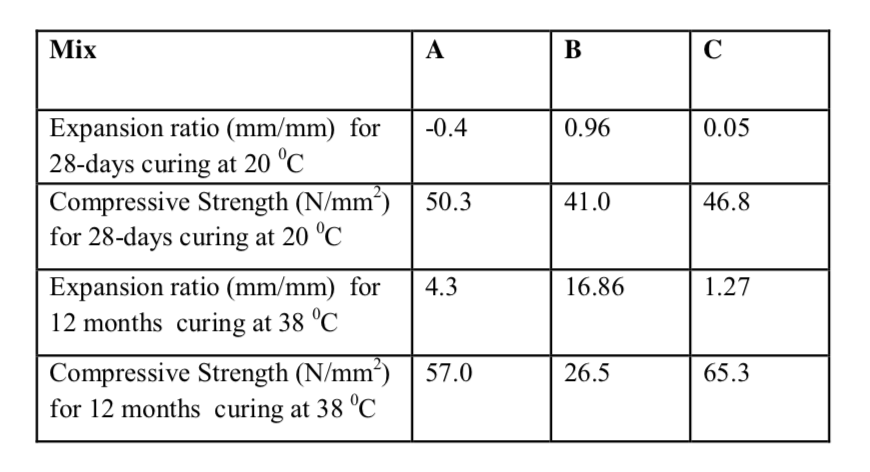
\includegraphics{Reference/temp1.png}
  \caption{}
  \label{}
\end{figure}

As seen in Table 3.1, the results reveal that compressive strength of Mix A is nearly 7.5\% higher than Mix C‟s (control mix) at 28 days due to no expansion in Mix A. However, compressive strength of Mix A is nearly 12.7\% less than Mix C‟s (control mix) at 12 months due to its greater expansion compared with expansion of Mix C. As for Mix B specimens with fused silica, they had the greatest expansion in the three mixes so that its compressive strength dropped nearly 12.4\% at cold water (20 0C) for 28 days with compared to Mix C. After stored at hot water (38 0C) for 12 months, the drop in strength of Mix B reached to nearly 59.4\% by showing severe cracking [Ahmed et al., 2003].As an another views, Cope and Slade observed an compressive strength increase in same mix (Mix A) and claimed that the curing of concrete including slowly reactive aggregate at high temperature doesn‟t affect overly on compressive strength of concrete at an early age or even after plenty time passes so compressive strength of Mix A can increase at 38 0C at this time [Cope & Slade, 1992]. Figure 3.1 reveals that a greater decrease in compressive strength was observed in Mix B compared with Mix A at any expansion percent due to different reaction rates for fused silia and Thames Vally sand permitting the hydration of cement to increase the compressive strength of concrete [Ahmed et al., 2003].


%TODO: Continue...

% TODO: GIANNINI(2012) P15-16 (Nothing Much)



 
